\subsection{Feature Selection \& Dimensionality Reduction Pipeline}
\label{subsec:feature_selection}

Having aggregated raw signal components through dynamic multi-level extraction, the computational pipeline immediately inherits a critically unsupportable density: specifically, extracting parameters per-channel across numerous frequency domains yields thousands of correlated variables (the ``curse of dimensionality''). In \texttt{pipeline/src/feature\_selection}, the architectural focus shifts mathematically to orthogonalizing these dimensions, structurally pruning redundant oscillatory artifacts to enhance inference clarity while fundamentally preserving pathological deviations.

\begin{figure}[htpb]
    \centering
    \resizebox{\textwidth}{!}{
    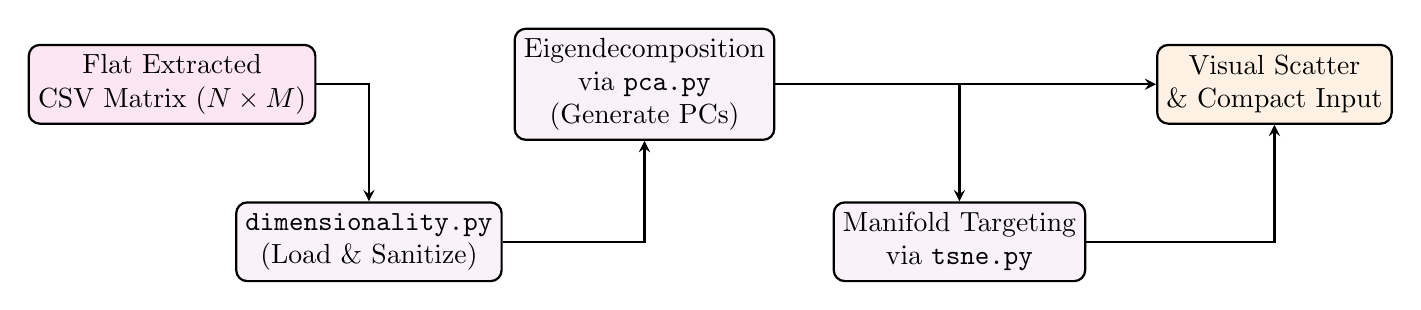
\begin{tikzpicture}[
        box/.style={draw, rectangle, rounded corners, align=center, minimum height=1cm, fill=violet!5, thick},
        arrow/.style={->, thick, -stealth}
    ]
        \node[box, fill=magenta!10] (input) at (0, 0) {Flat Extracted \\ CSV Matrix ($N \times M$)};
        
        \node[box] (dim) at (2.5, -2) {\texttt{dimensionality.py} \\ (Load \& Sanitize)};
        
        \node[box] (pca) at (6, 0) {Eigendecomposition \\ via \texttt{pca.py} \\ (Generate PCs)};
        
        \node[box] (tsne) at (10, -2) {Manifold Targeting \\ via \texttt{tsne.py}};
        
        \node[box, fill=orange!10] (output) at (14, 0) {Visual Scatter \\ \& Compact Input};

        \draw[arrow] (input.east) -| (dim.north);
        \draw[arrow] (dim.east) -| (pca.south);
        \draw[arrow] (pca.east) -| (tsne.north);
        \draw[arrow] (tsne.east) -| (output.south);
        \draw[arrow] (pca.east) -- (output.west);
    \end{tikzpicture}
    }
    \caption{Data flow governing dimensional reduction and visual embedding mapping from the raw CSV matrix to the final interpretable manifold.}
    \label{fig:feat_selection_process}
\end{figure}

\subsubsection{Matrix Loading and Scalar Structuring}
Centralized by \texttt{dimensionality.py}, the high-level input sequence natively handles the ingestion of massive CSV parameter dictionaries. Recognizing the inherently noisy context of neuro-metadata (file identities, timestamp strings, target categorizations), the sub-module executes string-masking algorithms that strip non-computable axes prior to standardizing scalar variances utilizing deterministic zero-mean unit-variance transformation: 
\begin{equation}
    x_{norm} = \frac{x - \mu}{\sigma}
\end{equation}
This normalisation phase resolves dominant-magnitude bias issues directly impacting topological projections (where features like high-voltage delta transients routinely crush nuanced spectral connectivity values).

\subsubsection{Eigen-Decomposition and Principal Components}
To explicitly isolate variance geometries linking cognitive disruption to sensor outputs, the \texttt{pca.py} sub-routine leverages customized NumPy routines to extract orthogonal Principal Components (PCs), instead of depending wholly on external libraries. Following the covariance matrix equation $C = \frac{1}{n-1} X^T X$, the routine dynamically shifts bases into eigen-vectors ($\mathbf{v}_i$) scaled against eigenvalues ($\lambda_i$).

Implementation design guarantees a deterministic output struct—the module returns defined \texttt{PCAResult} datatypes, tracking exact explained-variance ratios. Given early indications of Alzheimer's rest heavily on complex cross-channel variance, preserving 90-95\% cumulative dimensional variance allows models to reliably exclude random artifacts and target underlying continuous network abnormalities, dropping the matrix geometry from potentially tens of thousands of features down into highly resilient primary vectors \cite{acharya2018automated}. 

\subsubsection{t-SNE Embeddings for Empirical Spatial Mapping}
Linear variance structures like PCA inherently lose continuous relational mapping associated with non-linear, topological physiological clusters. To mitigate this mapping loss and present clinical proof-of-separation for underlying algorithms, \texttt{tsne.py} deploys t-Distributed Stochastic Neighbor Embedding (t-SNE) mapped explicitly out of the primary PCA outputs as an initialization base.

The t-SNE framework leverages a continuous Student's t-distribution for mapping lower-dimensional geometric spaces, aggressively separating divergent disease classifications while pulling tight pathological similarities together. Executed via iterative Kullback-Leibler (KL) divergence minimization, the script caches high-computation visual coordinates (e.g. 2D/3D spaces) directly into CSV files. This decision deliberately removes visualization load constraints away from inference runtimes while definitively validating that feature matrices mathematically separate baseline controls against cognitive impairment markers \textit{prior} to deep learning application.
